\section{Rotating/Twisting Bezier Splines}
\label{Chapter:SplineModelling}

    \subsection{The need of a Twisting Bezier splines}

    Conventional Bezier curves are commonly used to define outline fonts [cite] and digital calligraphy [cite] due to their ability to accurately trace [cite] the outline of scripts written with and without a broad edge tool [cite]. These curves can be easily manipulated [cite] and rendered [cite] on a computer screen as well as they can be printed on paper. However, in light of the underlaying problem, it is desired that a script is written using a conventional broad-edge tool by a robotic manipulator [cite] in a similar fashion a human artist would have used in order to preserve the essence of artistic norms [cite]. Separate techniques [cite] are needed to convert output of the outline or pitch curve functions to a format that a robot can directly use to for the required tool movement. Even though many of these techniques [cite] can promise accurate tracing, none of them can promise an exact tool movement that a human would like to use.

    In the most literal terms, beizer spline curves are sets of decimal values that define the graphical shape of certain mathematical functions [cite]. The input of these functions contains two dimensional points located in the frame of reference of the screen on which they are created and work as handles to control the shape of the curve. A user can physically relocate these curvature handles on the computer screen and the shape of the resulting spline will follow. The output of these mathematical functions is absolutely repeatable and can be linearly scaled to any units. Usually, a curve is made of up a lot of such lines each with its own set of input coefficients. Although these individual functions are continuous, there output can easily be discretized as closed paths made up of closely located two dimensional points with controllable resolution [cite]. This is exactly the kind of information required by most of computer graphics and printing drivers to render an output.

    Now, as effective as the bezier curves are for screen and paper printing, they still cannot tell how a physical tool should move on a piece of paper to create the desired output. The splines are just organic shaped paths with no thickness. To convert them into ink-mark, one way to interpret them is to consider them as a pitch line for a thick round tool tip. This technique is used by plotters [cite] and some hand writing replicators [cite] to produce a written script. However, only a few fonts [cite] can be replicated by this technique. The other technique is to fill the glyph by moving the tool continuously on a path computed by algorithms such as those used by CAD tools [cite] to fill in the area contained by the outline of the glyph using a round tip tool. The later can produce outputs that looks similar to broad-edge calligraphy but will still not be the same due to the visible tool paths that are not expected when using an actual broad edge tool.

    Conventionally, image processing is being used to extract data that can be used to create machine data. We, however, propose a difference; no matter how strong and robust image processing gets, we maintain that there is no alternative to the minor details only a real artist can observe and recreate. So a solution is needed that fulfils the technical needs as well as the artistic demands. One can virtually draw any kind of shape that can be represented on a two dimensional surface using the conventional bezier splines but it is not very intuitive to accurately reproduce the output of a broad-edge tool.

    Twisting bezier splines bridge this gaps by introducing a small but important innovation in the conventional bezier spline curves. Instead of working as outline curves, they directly record the pitch line of a twisting broad-edge tool stroke along-with the twist information of the tool. Their usage is just as intuitive as the conventional bezier splines and will be demonstrated in the next chapters, and the information they poses can not only be used to render the script back on the screen or a photo printer, but also be directly considered as machine data for robotic manipulators.

    On the other hand, for a particular glyph created with a broad edge, the twisting bezier spline curves not only trace the pitch lines of all the strokes but also the twist of the tool independent of the curvature. This is done by introducing another input to the curve function we call the ``Rotation/Twist'' handle. Just like the curvature handles represent the function inputs responsible to define the curvature, the rotation handles represent the inputs that controls the twist of the simulated broad-edge tool. Just like the conventional bezier splines, the functions of the twisting bezier splines can also be discretized and converted into a list of two dimensional list of points; a closed path to emulate the ink-mark of the broad edge tool, exactly the kind of data needed by the computer display drivers. This is how an artist can intuitively use the twisting curves not just to trace but also to create calligraphy that is not bound by any culture or language.

    The interesting part is that, logically, the twisting beizer splines are more near to the machine than they are to computer graphics data. To compute the list of the points needed to create a filled path that represents the ink-mark, a broad edge tool is emulated to be moving on the rotating spline with the twist also controlled by the spline. In actuality, the emulated tool is replaced by an actual tool that can be mounted on a robotic manipulator. The spline directly controls the position and twist of the tip of a tool which can directly be translated into machine movement codes. The rest of the process for painting involves inverse kinematics and is already handled by the robot controller.

    As discussed in section \ref{Chapter:Problem Statement}, the first part of the main problem is extracting digital machine data from the existing calligraphy specimens. Conventionally, image processing is being used to extract data that can be used to create machine data. We, however, propose a difference; no matter how strong and robust image processing gets, we maintain that there is no alternative to the minor details only a real artist can observe and recreate. So a solution is needed that fulfils the technical needs as well as the artistic demands.

    \subsection{Mathematical Model of a Rotating Bezier Spline}
    \subsubsection{The Conventional Bezier Spline}
         To describe how twisting splines work, we, once again, first describe it for a conventional bezier spline. Figure \ref{Fig:BezierSplines} shows an illustration of a spline path made up of several sub curves. Each curve section is only partly independent of the other. Figure \ref{Fig:BezierSplines} (a) shows the final shape of the curve without any construction elements. In Figure \ref{Fig:BezierSplines} (b), we explode different sections of the curve into smaller elements and show how they fit together to form the complete spline. There are five sections in this curve labeled $1$ through $5$. Figure \ref{Fig:BezierSplines} (c) shows an assembled form of these five sections. It also shows, what are called, anchors and construction handles. The anchor is the point that sits at the terminals of two adjacent curve sections. For instance, anchor point $A$  is connecting the sections $1$ and $2$. Like all the other anchors, this anchor also has two handles, $H_1$ and $H_2$, connected through a straight line passing through the anchor. The length of each handles, $\overline{AH_1}$  and $\overline{AH_2}$ on both sides of the anchor define the shape of the curve section on their respective side where as the orientation of line connecting both handles contributes to the shape on both the curve sections. This is how both sections become partly independent. For instance, handle $\overline{AH_1}$ contributes to the shape of curve segment $1$ and $\overline{AH_1}$ to section $2$.


        \begin{figure}
          \centering
          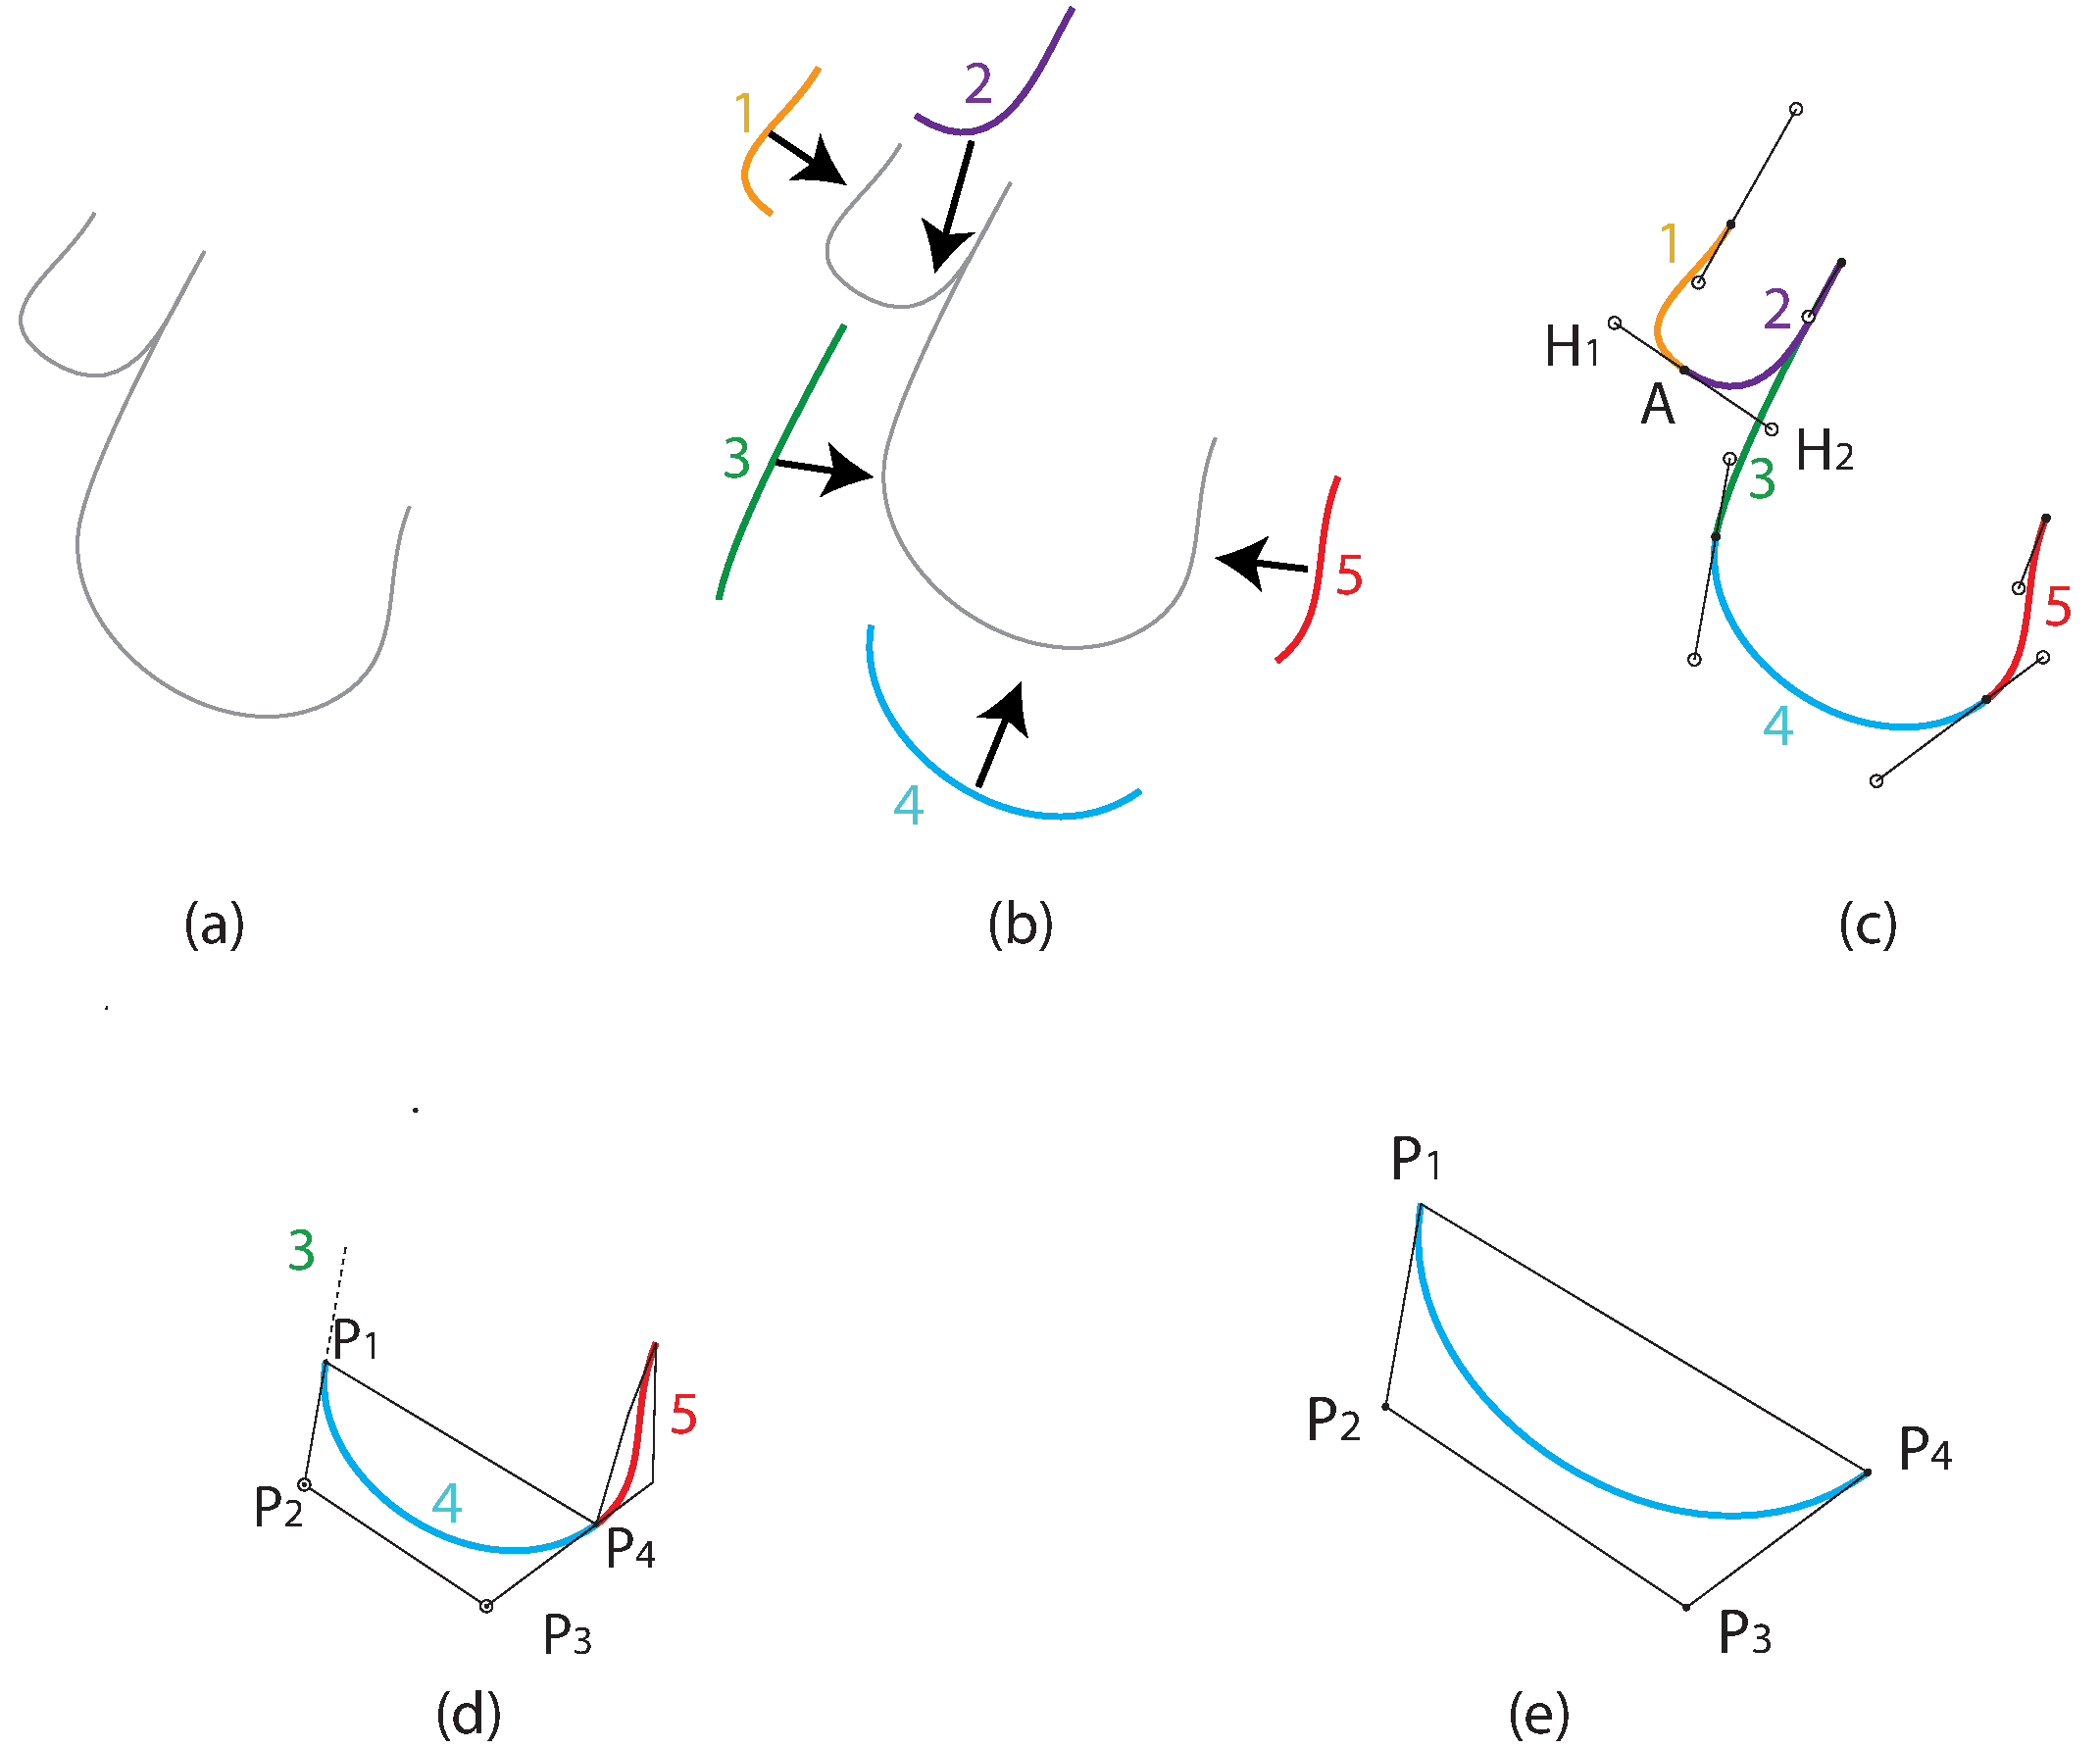
\includegraphics[width=0.9\textwidth]{../Images/BezierSplineCurve.pdf}
          \caption{An illustration showing the construction of Bezier Spline Curve. (a) A sample of a Bezier spline path (b) an exploded view of inner curves of the Bezier spline path (c) Handles that control the shape of the two adjacent sub curves (d) and (e) Construction polygon of the sub curve.
          } \label{Fig:BezierSplines}
        \end{figure}

        Now, it may look like the shapes defined in this way are pretty organic but in fact, the whole shape is defined by simple mathematical equations. Figure \ref{Fig:BezierSplines} (d) focuses on section $4$ and $5$ of the curve and also shows a polygon defined by the points $P_1$, $P_2$, $P_3$ and  $P_4$. It must be noted that the points $P_1$ and $P_4$ of this polygon are also the anchor point between sections $3$, $4$ and $5$. Take section $4$ for example here. The polygon mathematically defines the complete shape of this curve part. If $P_{spline}$ is a point on the section $4$, with coordinates $x$ and $y$ in a cartesian plane with some origin, it is defined as
         \begin{equation}
         P_{spline}=P_b×f+P_a×(1 -f).
         \end{equation}
where,
\begin{equation}
P_a=P_{23}×f+P_{12}×(1 -f)
\end{equation}
and
\begin{equation}
P_b=P_{34}×f+P_{23}×(1 -f)
\end{equation}
where,
\begin{eqnarray}
P_{12}&=&P_2×f+P_1×(1 -f), \\
P_{23}&=&P_3×f+P_2×(1 -f)
\end{eqnarray}
and
\begin{equation}
P_{34}=P_4×f+P_3×(1 -f)
\end{equation}
for an $f$ in the range $[0, 1]$.

It can also be proved that the side segments of the polygon $\overline{P_1 P_2}$ and $\overline{P_3 P_4}$ are tangent to the curve at the point they meet it at $P_1$ and $P_4$ respectively.


\subsubsection{Twist/Rotation Handle}
    On top of the conventional Bezier splines that work around anchor points that have curvature handles, we add a “Rotation”/”Twist” handle in the anchor and a thickness parameter to the whole curve. A rotation handle is similar to the curvature handle discussed earlier, except it does not have any effect on the shape of the curve. The thickness parameter defines the size of a flat line segment  centered on $P_{spline}$ and sweeping on it. The orientation of this sweeping line is the same as the angle between the twist handle and the respective anchor. See Figure \ref{Fig:RotatingBezierSplines} (a) that shows rotation handles added in the example under discussion. It must be noted that the curvature of the spline remains the same after adding twist handles that are lying horizontally yet. We then add thickness to the curve in Figure \ref{Fig:RotatingBezierSplines} (b). The resulting curve may look a little out of order but it is normal. This is because the rotation handles are lying on their default position. The twist handles may be given some length but it is insignificant since the twist of the curve will only take the value of the angle the handle subtends about the anchor. Figure \ref{Fig:RotatingBezierSplines} (c) shows the final form of the twisting bezier spline after the twist handles have been iteratively moved to position that give the spline the desired look.

        \begin{figure}
          \centering
          \includegraphics[width=0.9\textwidth]{../Images/AddingTwist_300PPI.jpg}
          \caption{A normal bezier spline is given the rotation handle. (a) rotation handles are shown on the anchors. (b) The rotation handles are given a visible thickness value. (c) The rotation handles are moved to give the spline the desired shape.
          } \label{Fig:RotatingBezierSplines}
        \end{figure}

    In simpler words, it’s similar to sweeping a pen centered on the actual spline while twisting it uniformly and continuously about its own axis according to the equation
    \begin{equation}
    \theta_{twist}=\theta_A  (1-f)+ \theta_B
    \end{equation}
    where $f$ is the same factor that was used to define $P_{spline}$ and $\theta_A$ and $\theta_B$ are the angles between the first and the second anchor and their rotation handles respectively. It may be noted that since each anchor is connecting two adjacent sub curves, the ending angle of the sweeping line at the end of the first curve is always the same at the beginning of the later. This visually hides the transition of the twisting curve from one sub curve to the other.

    It must also be noted that the angle of rotation handle cannot be constrained in a $2\pi$ domain. Instead, it is completely unbounded, and the sweeping pen may actually take multiple turns both clockwise and anticlockwise while moving on a single curve section as well as the whole curve. When the idea of the twisting splines was first conceived, it wasn’t envisaged that the angle had to be taken like in this scheme. Special care had to be taken in order to graphically read a continuous angle from the user.

    See Appendix \ref{Appendix:CodeSnippets} which compiles the rectangular coordinates of all the anchors of the rotating bezier spline shown formatted in a manner that Gregor can interpret. In chapter \ref{Chapter:Gregor}, we discuss in detail ``Gregor'', the tool that uses this data to save the created splines.

\subsection{Conversion of Existing Calligraphy Artwork}
Instead of using image processing to extract data from existing scans and photographs of the artworks, using rotating Bezier splines we can now include the artists in the process. Just like any other computer-based graphics design application, we share a proof of concept tool to create, modify, save, and reload rotating Bezier splines. The tool can be downloaded online [link to source][link to user manual] and features an easy to use interface and the tools needed to conveniently create, modify new splines and trace existing ones.

\subsection{Machine Data Generation}
\label{ExplorationPoints1}
The rotating spline curves are themselves emulated ink-marks of a broad edge marking tool. This is the reason extracting machine data and even G-codes from them becomes natural. If the flat side of the tool is assumed to be entirely touching the writing surface, the minimum information required to draw a stroke trickles down to the line on which the pen must move and the twist of the pen in world coordinates. Minus the information about a three dimensional reference system, this is exactly the information a rotating Bezier spline contains once an artist has drawn them on the computer screen. In other words, to call the rotation Bezier splines the machine data, the following assumptions must be made:
\begin{itemize}
	\item The flat tip of a broad edge tool is always completely touching the drawing area.
	\item The inclination of the pen with respect to the drawing area or with respect to the direction of the drawing is either normal or always fixed at an angle and is set by the machine.
	\item To produce thinner strokes, another spline will be used. This means that the machine would have to use multiple tools for such splines.
	\item The axial pressure the pen inserts on the drawing board while drawing is also fixed and is set by the machine as well.
\end{itemize}

It is now obvious that to remove the limitations of fixed angles and pressure values, one can add more handles similar to the rotation handle. A set of bi-directional inclination handles can be added right away with a three-dimensional pen position visualizer to assist the artist determine what angle they want to keep the pen at while drawing a specific stroke. The pressure angle, however, would not be recommended without interfacing some hardware that lets the artist feel the pen pressure in real time before setting a handle value. This can be done using a pressure sensitive digital pen or writing tablets [16-18]. These expansions alone are in themselves worthy of research projects that rivals the scope of the current one.
